\chapter{链表}

\section{链表}

\subsection{单向链表(Singly Linked List)}

为避免元素的移动,采用线性表的另一种存储方式:链式存储结构。链表是一种在物理上非连续、非顺序的数据结构,由若干结点(node)所组成。 \\

单向链表的每一个结点又包含两部分,一部分是存放数据的数据域data,另一部分是指向下一个结点的指针域next。结点可以在运行时动态生成。

\vspace{-0.5cm}

\begin{lstlisting}[language=C]
typedef struct Node {
    dataType data;          // 数据域
    struct Node *next;		// 指针域
} Node;
\end{lstlisting}

链表的第一个结点被称为头结点,最后一个节点被称为尾结点,尾结点的next指针指向空NULL。 \\

\begin{figure}[H]
	\centering
	\begin{tikzpicture}[list/.style={rectangle split, rectangle split parts=2,
					draw, rectangle split horizontal}, >=stealth, start chain]
		\node[list,on chain] (A) {data};
		\node[list,on chain] (B) {data};
		\node[list,on chain] (C) {data};
		\node[on chain,draw,inner sep=6pt] (D) {};
		\draw (D.north east) -- (D.south west);
		\draw (D.north west) -- (D.south east);
		\draw[*->] let \p1 = (A.two), \p2 = (A.center) in (\x1,\y2) -- (B);
		\draw[*->] let \p1 = (B.two), \p2 = (B.center) in (\x1,\y2) -- (C);
		\draw[*->] let \p1 = (C.two), \p2 = (C.center) in (\x1,\y2) -- (D);
	\end{tikzpicture}
	\caption{单向链表}
\end{figure}

与数组按照下标来随机寻找元素不同,对于链表的其中一个结点A,只能根据结点A的next指针来找到该结点的下一个结点B,再根据结点B的next指针找到下一个节点C…… \\

数组在内存中的存储方式是顺序存储,链表在内存中的存储方式则是随机存储。链表采用了见缝插针的方式,每一个结点分布在内存的不同位置,依靠next指针关联起来。这样可以灵活有效地利用零散的碎片空间。

\subsection{双向链表(Doubly Linked List)}

那么,通过链表的一个结点,如何能快速找到它的前一个结点呢?要想让每个结点都能回溯到它的前置结点,可以使用双向链表。 \\

双向链表比单向链表稍微复杂一点,它的每一个结点除了拥有data和next指针,还拥有指向前置结点的prev指针。 \\

\begin{figure}[H]
	\centering
	\begin{tikzpicture}[list/.style={rectangle split, rectangle split parts=3,
					draw, rectangle split horizontal}, >=stealth, start chain]
		\node[on chain,draw,inner sep=6pt] (NULL1) {};
		\node[list,on chain] (A) {prev \nodepart{second} data \nodepart{third} next};
		\node[list,on chain] (B) {prev \nodepart{second} data \nodepart{third} next};
		\node[list,on chain] (C) {prev \nodepart{second} data \nodepart{third} next};
		\node[on chain,draw,inner sep=6pt] (NULL2) {};
		\draw (NULL1.north east) -- (NULL1.south west);
		\draw (NULL1.north west) -- (NULL1.south east);
		\draw (NULL2.north east) -- (NULL2.south west);
		\draw (NULL2.north west) -- (NULL2.south east);
		\draw[<-] let \p1 = (A.west), \p2 = (A.center) in (NULL1) -- (\x1,\y2);
		\draw[<->] let \p1 = (A.east), \p2 = (A.center) in (\x1,\y2) -- (B);
		\draw[<->] let \p1 = (B.east), \p2 = (B.center) in (\x1,\y2) -- (C);
		\draw[->] let \p1 = (C.east), \p2 = (C.center) in (\x1,\y2) -- (NULL2);
	\end{tikzpicture}
	\caption{双向链表}
\end{figure}

单向链表只能从头到尾遍历,只能找到后继,无法找到前驱,因此遍历的时候不会死循环。而双向链表需要多分配一个指针的存储空间,每个结点有两个指针,分别指向直接前驱和直接后继。

\subsection{循环链表(Circular Linked List)}

除了单向链表和双向链表以外,还有循环链表。对于单向循环链表,尾结点的next指针指向头结点。对于双向循环链表,尾结点的next指针指向头结点,并且头结点的prev指针指向尾结点。 \\

\begin{figure}[H]
	\centering
	\begin{tikzpicture}[
			list/.style={
					rectangle split,
					rectangle split parts=2,
					draw,
					rectangle split horizontal
				},
			dotarrow/.style={Circle-Stealth},
			start chain
		]
		\node[list,on chain] (A) {data};
		\node[list,on chain] (B) {data};
		\node[list,on chain] (C) {data};
		\draw[dotarrow] (A.two |- A.center) -- (B);
		\draw[dotarrow] (B.two |- B.center)  -- (C);
		\draw[dotarrow] (C.two |- C.center) to[out=-20,in=190,distance=4cm] (A);
	\end{tikzpicture}
	\caption{单向循环链表}
\end{figure}

\begin{figure}[H]
	\centering
	\begin{tikzpicture}[list/.style={
					rectangle split,
					rectangle split parts=3,
					draw,
					rectangle split horizontal
				},
			dotarrow/.style={Circle-Stealth},
			start chain]
		\node[list,on chain] (A) {prev \nodepart{second} data \nodepart{third} next};
		\node[list,on chain] (B) {prev \nodepart{second} data \nodepart{third} next};
		\node[list,on chain] (C) {prev \nodepart{second} data \nodepart{third} next};

		\draw[dotarrow] (A.center -| A.west) to[out=-220,in=20,distance=2cm] (C.north);
		\draw[<->] let \p1 = (A.east), \p2 = (A.center) in (\x1,\y2) -- (B);
		\draw[<->] let \p1 = (B.east), \p2 = (B.center) in (\x1,\y2) -- (C);
		\draw[dotarrow] (C.east |- C.center) to[out=-20,in=220,distance=2cm] (A.south);
	\end{tikzpicture}
	\caption{双向循环链表}
\end{figure}

\newpage

\section{链表的增删改查}

\subsection{查找结点}

在查找元素时,链表不像数组那样可以通过下标快速进行定位,只能从头结点开始向后一个一个结点逐一查找。 \\

链表中的数据只能按顺序进行访问,最坏的时间复杂度是$ O(n) $。 \\

\mybox{查找结点}

\begin{lstlisting}[language=C]
Node* search(List *head, dataType val) {
    // 查找元素位置
    Node *temp = head;
    while(temp) {
        if(temp->data == val) {
            return temp;
        }
        temp = temp->next;
    }
    return NULL;        // 未找到
}
\end{lstlisting}

\subsection{更新结点}

如果不考虑查找结点的过程,链表的更新过程会像数组那样简单,直接把旧数据替换成新数据即可。 \\

\mybox{更新结点}

\begin{lstlisting}[language=C]
void replace(List *head, int pos, dataType val) {
    // 找到元素位置
    Node *temp = head;
    for(int i = 0; i < pos; i++) {
        temp = temp->next;
    }
    temp->data = val;
}
\end{lstlisting}

\subsection{插入结点}

链表插入结点,分为3种情况:

\subsubsection{尾部插入}

把最后一个结点的next指针指向新插入的结点。

\begin{figure}[H]
	\centering
	\begin{tikzpicture}[node distance=2cm, auto, scale=1,
			every node/.style={scale=1}]
		\node[head, label=below:head] (head) {};
		\node[data, right of=head] (A) {\data};
		\node[above of=A,node distance=0.5cm,label=above:a1] (a1){};
		\node[data, right of=A] (B) {\data};
		\node[above of=B,node distance=0.5cm,label=above:a2] (a2){};
		\node[data, right of=B] (C) {\data};
		\node[above of=C,node distance=0.5cm,label=above:a3] (a3){};
		\node[data, right of=C, xshift=0.1cm] (D) {\data};%, xshift=1.5cm
		\node[above of=D,node distance=0.5cm,label=above:a4] (a4){};
		\node[data, right of=D] (E) {\data};
		\node[above of=E,node distance=0.5cm,label=above:a5] (a5){};
		\node[data, right of=E] (last) {data \nodepart{second} \texttt{NULL}};
		\node[above of=last,node distance=0.5cm,label=above:new] (new){};

		\draw[fill] (head.center) circle (0.05);

		\path[ptr] (head.center) --++(right:7.5mm) |- (A.text west);
		\draw[fill] ($(A.south)!0.5!(A.text split)$) circle (0.05);
		\draw[ptr] ($(A.south)!0.5!(A.text split)$) --++(right:10mm) |- (B.text west);
		\draw[fill] ($(B.south)!0.5!(B.text split)$) circle (0.05);
		\draw[ptr] ($(B.south)!0.5!(B.text split)$) --++(right:10mm) |- (C.text west);
		\draw[fill] ($(C.south)!0.5!(C.text split)$) circle (0.05);
		\draw[ptr] ($(C.south)!0.5!(C.text split)$) --++(right:10mm) |- (D.text west);
		\draw[fill] ($(D.south)!0.5!(D.text split)$) circle (0.05);

		\draw[fill] ($(D.south)!0.5!(D.text split)$) circle (0.05);
		\draw[ptr] ($(D.south)!0.5!(D.text split)$) --++(right:10mm) |- (E.text west);
		\draw[fill] ($(E.south)!0.5!(E.text split)$) circle (0.05);
		\draw[ptr] ($(E.south)!0.5!(E.text split)$) --++(right:10mm) |- (last.text west);
	\end{tikzpicture}
	\caption{尾部插入}
\end{figure}

\subsubsection{头部插入}

先把新结点的next指针指向原先的头结点,再把新结点设置为链表的头结点。

\begin{figure}[H]
	\centering
	\begin{tikzpicture}[node distance=2cm, auto, scale=1,
			every node/.style={scale=1}]
		\node[head, label=below:head, xshift=-0.5cm] (head) {};
		\node[data, right of=head] (A) {\data};
		\node[above of=A,node distance=0.5cm,label=above:a1] (a1){};
		\node[data, right of=A] (B) {\data};
		\node[above of=B,node distance=0.5cm,label=above:a2] (a2){};
		\node[data, right of=B] (C) {\data};
		\node[above of=C,node distance=0.5cm,label=above:a3] (a3){};
		\node[data, below of=head, xshift=0.6cm, yshift=0.5cm] (NEW) {\data};
		\node[above of=NEW,node distance=0.3cm,label=above:new] (new){};
		\node[data, right of=C, xshift=0.1cm] (D) {\data};%, xshift=1.5cm
		\node[above of=D,node distance=0.5cm,label=above:a4] (a4){};
		\node[data, right of=D] (E) {\data};
		\node[above of=E,node distance=0.5cm,label=above:a5] (a5){};
		\node[data, right of=E] (last) {data \nodepart{second} \texttt{NULL}};
		\node[above of=last,node distance=0.5cm,label=above:a6] (a6){};

		\draw[fill] (head.center) circle (0.05);

		\path[ptr] (head.center) --++(left:7.5mm) |- (NEW.text west);
		\draw[fill] ($(NEW.south)!0.5!(NEW.text split)$) circle (0.05);
		\draw[ptr] ($(NEW.south)!0.5!(NEW.text split)$) --++(right:6mm) |- (A.text west);
		\draw[fill] ($(A.south)!0.5!(A.text split)$) circle (0.05);
		\draw[ptr] ($(A.south)!0.5!(A.text split)$) --++(right:10mm) |- (B.text west);
		\draw[fill] ($(B.south)!0.5!(B.text split)$) circle (0.05);
		\draw[ptr] ($(B.south)!0.5!(B.text split)$) --++(right:10mm) |- (C.text west);
		\draw[fill] ($(C.south)!0.5!(C.text split)$) circle (0.05);
		\draw[ptr] ($(C.south)!0.5!(C.text split)$) --++(right:10mm) |- (D.text west);
		\draw[fill] ($(D.south)!0.5!(D.text split)$) circle (0.05);
		\draw[fill] ($(D.south)!0.5!(D.text split)$) circle (0.05);
		\draw[ptr] ($(D.south)!0.5!(D.text split)$) --++(right:10mm) |- (E.text west);
		\draw[fill] ($(E.south)!0.5!(E.text split)$) circle (0.05);
		\draw[ptr] ($(E.south)!0.5!(E.text split)$) --++(right:10mm) |- (last.text west);
	\end{tikzpicture}
	\caption{头部插入}
\end{figure}

\subsubsection{中间插入}

先把新结点的next指针指向插入位置的结点,再将插入位置的前置结点的next指针指向新结点。

\begin{figure}[H]
	\centering
	\begin{tikzpicture}[node distance=2cm, auto, scale=1,
			every node/.style={scale=1}]
		\node[head, label=below:head] (head) {};
		\node[data, right of=head] (A) {\data};
		\node[above of=A,node distance=0.5cm,label=above:a1] (a1){};
		\node[data, right of=A] (B) {\data};
		\node[above of=B,node distance=0.5cm,label=above:a2] (a2){};
		\node[data, right of=B] (C) {\data};
		\node[above of=C,node distance=0.5cm,label=above:a3] (a3){};
		\node[data, below of=C, xshift=0.8cm, yshift=0.5cm] (NEW) {\data};
		\node[above of=NEW,node distance=0.3cm,label=above:new] (new){};
		\node[data, right of=C, xshift=0.1cm] (D) {\data};%, xshift=1.5cm
		\node[above of=D,node distance=0.5cm,label=above:a4] (a4){};
		\node[data, right of=D] (E) {\data};
		\node[above of=E,node distance=0.5cm,label=above:a5] (a5){};
		\node[data, right of=E] (last) {data \nodepart{second} \texttt{NULL}};
		\node[above of=last,node distance=0.5cm,label=above:a6] (a6){};

		\draw[fill] (head.center) circle (0.05);

		\path[ptr] (head.center) --++(right:7.5mm) |- (A.text west);
		\draw[fill] ($(A.south)!0.5!(A.text split)$) circle (0.05);
		\draw[ptr] ($(A.south)!0.5!(A.text split)$) --++(right:10mm) |- (B.text west);
		\draw[fill] ($(B.south)!0.5!(B.text split)$) circle (0.05);
		\draw[ptr] ($(B.south)!0.5!(B.text split)$) --++(right:10mm) |- (C.text west);
		\draw[fill] ($(C.south)!0.5!(C.text split)$) circle (0.05);

		\draw[ptr] ($(C.south)!0.5!(C.text split)$) |- (NEW.text west);
		\draw[fill] ($(NEW.south)!0.5!(NEW.text split)$) circle (0.05);
		\draw[ptr] ($(NEW.south)!0.5!(NEW.text split)$) --++(right:6mm) |- (D.text west);
		\draw[fill] ($(D.south)!0.5!(D.text split)$) circle (0.05);
		\draw[ptr] ($(D.south)!0.5!(D.text split)$) --++(right:10mm) |- (E.text west);
		\draw[fill] ($(E.south)!0.5!(E.text split)$) circle (0.05);
		\draw[ptr] ($(E.south)!0.5!(E.text split)$) --++(right:10mm) |- (last.text west);
	\end{tikzpicture}
	\caption{中间插入}
\end{figure}

只要内存空间允许,能够插入链表的元素是无穷无尽的,不需要像数组考虑扩容的问题。如果不考虑插入之前的查找元素的过程,只考虑纯粹的插入操作,时间复杂度是$ O(1) $。

\subsection{删除结点}

链表的删除操作也分3种情况:

\subsubsection{尾部删除}

把倒数第二个结点的next指针指向空。

\begin{figure}[H]
	\centering
	\begin{tikzpicture}[node distance=2cm, auto, scale=1,
			every node/.style={scale=1}]
		\node[head, label=below:head] (head) {};
		\node[data, right of=head] (A) {\data};
		\node[above of=A,node distance=0.5cm,label=above:a1] (a1){};
		\node[data, right of=A] (B) {\data};
		\node[above of=B,node distance=0.5cm,label=above:a2] (a2){};
		\node[data, right of=B] (C) {\data};
		\node[above of=C,node distance=0.5cm,label=above:a3] (a3){};
		\node[data, right of=C, xshift=0.1cm] (D) {\data};
		\node[above of=D,node distance=0.5cm,label=above:a4] (a4){};
		\node[data, right of=D] (E) {\data};
		\node[above of=E,node distance=0.5cm,label=above:a5] (a5){};

		\draw[fill] (head.center) circle (0.05);

		\path[ptr] (head.center) --++(right:7.5mm) |- (A.text west);
		\draw[fill] ($(A.south)!0.5!(A.text split)$) circle (0.05);
		\draw[ptr] ($(A.south)!0.5!(A.text split)$) --++(right:10mm) |- (B.text west);
		\draw[fill] ($(B.south)!0.5!(B.text split)$) circle (0.05);
		\draw[ptr] ($(B.south)!0.5!(B.text split)$) --++(right:10mm) |- (C.text west);
		\draw[fill] ($(C.south)!0.5!(C.text split)$) circle (0.05);
		\draw[ptr] ($(C.south)!0.5!(C.text split)$) --++(right:10mm) |- (D.text west);
		\draw[fill] ($(D.south)!0.5!(D.text split)$) circle (0.05);

		\draw[fill] ($(D.south)!0.5!(D.text split)$) circle (0.05);
		\draw[ptr,red] ($(D.south)!0.5!(D.text split)$) -- (8.1,-1.7) -- (11.5,-1.7) -- (last.text west);
		\draw[fill] ($(E.south)!0.5!(E.text split)$) circle (0.05);

		\draw (12.3,0.3) node {NULL};

		\draw[-, red] (9.3,1) -- (11,-1); 
	\end{tikzpicture}
	\caption{尾部删除}
\end{figure}

\subsubsection{头部删除}

把链表的头结点设置为原先头结点的next指针。

\begin{figure}[H]
	\centering
	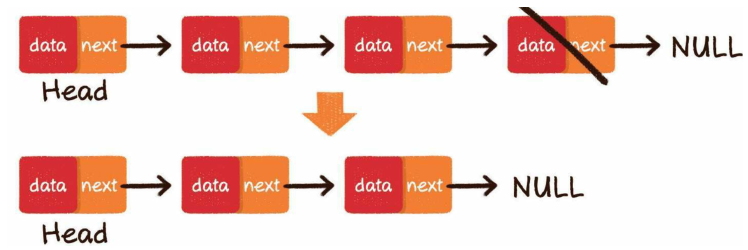
\includegraphics[scale=0.8]{img/C3/3-2/1.png}
\end{figure}

\subsubsection{中间删除}

把要删除的结点的前置结点的next指针,指向要删除结点的下一个结点。

\begin{figure}[H]
	\centering
	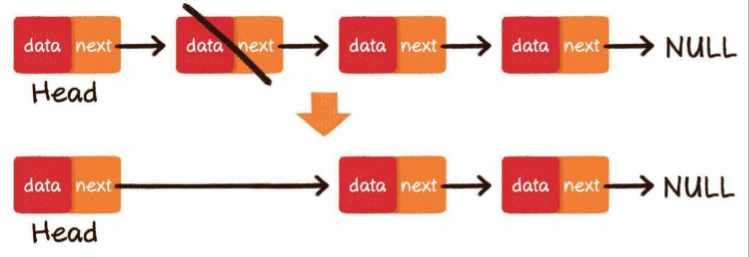
\includegraphics[scale=0.5]{img/C3/3-2/2.png}
\end{figure}

许多高级语言,如Java,拥有自动化的垃圾回收机制,所以不用刻意去释放被删除的结点,只要没有外部引用指向它们,被删除的结点会被自动回收。 \\

如果不考虑删除操作之前的查找的过程,只考虑纯粹的删除操作,时间复杂度是$ O(1) $。

\newpage

\section{带头结点的链表}

\subsection{带头结点的链表}

为了方便链表的插入、删除操作,在链表加上头结点之后,无论链表是否为空,头指针始终指向头结尾。因此对于空表和非空表的处理也统一了,方便了链表的操作,也减少了程序的复杂性和出现bug的机会。 \\

\mybox{插入结点}

\begin{lstlisting}[language=C]
void insert(List *head, int pos, dataType val) {
    Node *newNode = (Node *)malloc(sizeof(Node));
    newNode->data = val;
    newNode->next =  NULL;
    
    // 找到插入位置
    Node *temp = head;
    for(int i = 0; i < pos; i++) {
        temp = temp->next;
    }
    newNode->next = temp->next;
    temp->next = newNode;
}
\end{lstlisting}

\vspace{0.5cm}

\mybox{删除结点}

\begin{lstlisting}[language=C]
void delete(List *head, int pos) {
    Node *temp = head;
    for(int i = 0; i < pos; i++) {
        temp = temp->next;
    }
    Node *del = temp->next;
    temp->next = del->next;
    free(del);
    del = NULL;
}
\end{lstlisting}

\subsection{数组VS链表}

数据结构没有绝对的好与坏,数组和链表各有千秋。

\begin{table}[H]
	\centering
	\setlength{\tabcolsep}{5mm}{
		\begin{tabular}{|c|l|l|}
			\hline
			\textbf{比较内容} & \textbf{数组}          & \textbf{链表}                \\
			\hline
			基本              & 一组固定数量的数据项   & 可变数量的数据项             \\
			\hline
			大小              & 声明期间指定           & 无需指定,执行期间增长或收缩 \\
			\hline
			存储分配          & 元素位置在编译期间分配 & 元素位置在运行时分配         \\
			\hline
			元素顺序          & 连续存储               & 随机存储                     \\
			\hline
			访问元素          & 直接访问:索引、下标   & 顺序访问:指针遍历           \\
			\hline
			插入/删除         & 速度慢                 & 快速、高效                   \\
			\hline
			查找              & 线性查找、二分查找     & 线性查找                     \\
			\hline
			内存利用率        & 低效                   & 高效                         \\
			\hline
		\end{tabular}
	}
	\caption{数组VS链表}
\end{table}

数组的优势在于能够快速定位元素,对于读操作多、写操作少的场景来说,用数组更合适一些。 \\

相反,链表的优势在于能够灵活地进行插入和删除操作,如果需要频繁地插入、删除元素,用链表更合适一些。